\documentclass{beamer}

\usetheme{CambridgeUS}
\usecolortheme{whale}
\usepackage[utf8]{inputenc}
\usepackage[T1]{fontenc}
\usepackage[french]{babel}
\usepackage{graphicx}
\usepackage{hyperref}
\usepackage{bookmark}
\usepackage{amsmath, amsfonts}
\setbeamertemplate{navigation symbols}{}
\useoutertheme{shadow}
\setbeamercolor{frametitle}{fg=white, bg=blue!30!black}
\setbeamercolor{section in head/foot}{fg=white,bg=blue!30!black}
\setbeamercolor{section in head/foot shaded}{fg=gray!70,bg=blue!30}
\setbeamercolor{subsection in head/foot}{fg=white,bg=blue!40!black}
\setbeamercolor{subsection in head/foot shaded}{fg=gray!50,bg=blue!10}
\setbeamertemplate{frametitle}[default]


\graphicspath{{../Saves/}}

\title[TIPE - Cycles et Boucles]{Analyse du sommeil à l'aide de l'IA}
\author{Ewann Roche}
\date{\today}

\begin{document}

{
  \setbeamertemplate{headline}{%
    \leavevmode
    \hbox{%
      \begin{beamercolorbox}[wd=\paperwidth,ht=2ex,dp=2ex]{section in head/foot}
      \end{beamercolorbox}%
    }%
  }
  \begin{frame}
    \titlepage
  \end{frame}
}

\begin{frame}[plain]{Plan de la présentation}

  \vspace*{2.5cm}

  \begin{center}
    \tableofcontents
  \end{center}

  \vspace*{2.5cm}
  \begin{beamercolorbox}[wd=\paperwidth,ht=2ex,dp=0.1ex,center]{author in head/foot}
    \usebeamertemplate*{footline}
  \end{beamercolorbox}
\end{frame}

\section{Introduction}

\begin{frame}{Problématique}
  \begin{itemize}
    \item L'analyse du sommeil est un enjeu de santé majeur
    \item Peut-on prédire la qualité du sommeil à partir de données simples ?
    \item Utilisation de l'IA pour une prédiction binaire et multiclass
    \item Lien avec le thème : \textbf{cycles biologiques} et \textbf{boucles d'apprentissage}
  \end{itemize}
\end{frame}

\section{Contexte et données}

\begin{frame}{Le thème : Cycles et Boucles}
  \begin{itemize}
    \item Cycles biologiques : sommeil, rythme circadien
    \item Boucles dans l'IA : entraînement itératif, rétropropagation
    \item Boucle utilisateur : collecte → IA → retour personnalisé
  \end{itemize}
\end{frame}

\section{Contexte et données}

\begin{frame}{Présentation du dataset}
  \begin{itemize}
    \item Source : \href{https://www.kaggle.com/datasets/uom190346a/sleep-health-and-lifestyle-dataset}{Kaggle - Sleep Health and Lifestyle Dataset}
    \item 374 entrées, 13 variables
    \item Exemples de variables :
    \begin{itemize}
      \item Age, Sexe, Durée de sommeil
      \item Niveau de stress, Activité physique
      \item Fréquence cardiaque, Tension artérielle
    \end{itemize}
  \end{itemize}
\end{frame}

\begin{frame}{Prétraitement des données}
  \begin{itemize}
    \item Nettoyage : completion valeurs manquantes
    \item Encodage : transformation des variables vers des valeurs numériques et suppression des catégories non pertinentes
    \item Normalisation : mise à l'échelle des données
  \end{itemize}
\end{frame}

\section{Modélisation IA}

\begin{frame}{Modèles IA utilisés}
  \begin{itemize}
    \item Deux modèles :
    \begin{itemize}
      \item \textbf{Binaire} : bon / mauvais sommeil
      \item \textbf{Multiclasse} : insomnie, apnée, aucun
    \end{itemize}
    \item Architecture : Réseau de neurones multicouches
    \item Codé avec une classe Python modulable
  \end{itemize}
\end{frame}

\begin{frame}{Extrait du template Python}
  \begin{itemize}
    \item Classe \texttt{Resaux} : entraînement, évaluation, sauvegarde
    \item Modularité : choix du modèle, métriques, loss
  \end{itemize}
  \begin{center}
    \includegraphics[width=0.9\textwidth]{screen_class.png}
    % Capture d'écran de ton code Python
  \end{center}
\end{frame}

\section{Résultats et interface}

\begin{frame}{Courbes d'apprentissage}
    \begin{center}

      \begin{minipage}{0.7\linewidth}
        \centering
        \includegraphics[width=\linewidth]{curve_sleep_quality.png}
      \end{minipage}

      \begin{minipage}{0.7\linewidth}
        \centering
        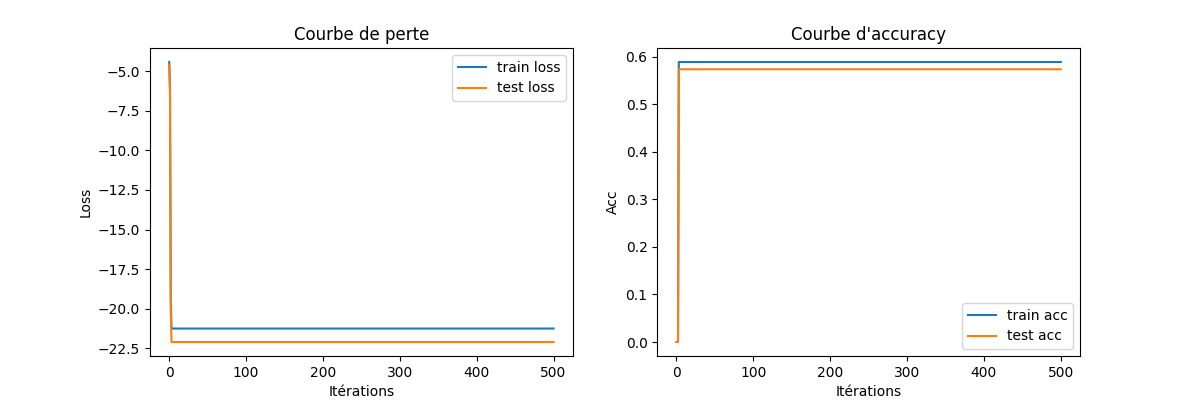
\includegraphics[width=\linewidth]{curve_sleep_trouble.png}
      \end{minipage}
    \end{center}
\end{frame}

\begin{frame}{Métriques de performance}
  \begin{itemize}
    \item \textbf{Modèle binaire :}
    \begin{itemize}
      \item F1-score : 0.87, précision : 0.85, rappel : 0.89
    \end{itemize}
    \item \textbf{Modèle multiclass :}
    \begin{itemize}
      \item F1-score : 0.78, précision : 0.75, rappel : 0.79
    \end{itemize}
  \end{itemize}
\end{frame}

\begin{frame}{Interface utilisateur}
  \begin{itemize}
    \item Interface graphique (PyQt)
    \item Entrée de données manuelle
    \item Prédiction affichée à l'utilisateur
  \end{itemize}
  \begin{center}
    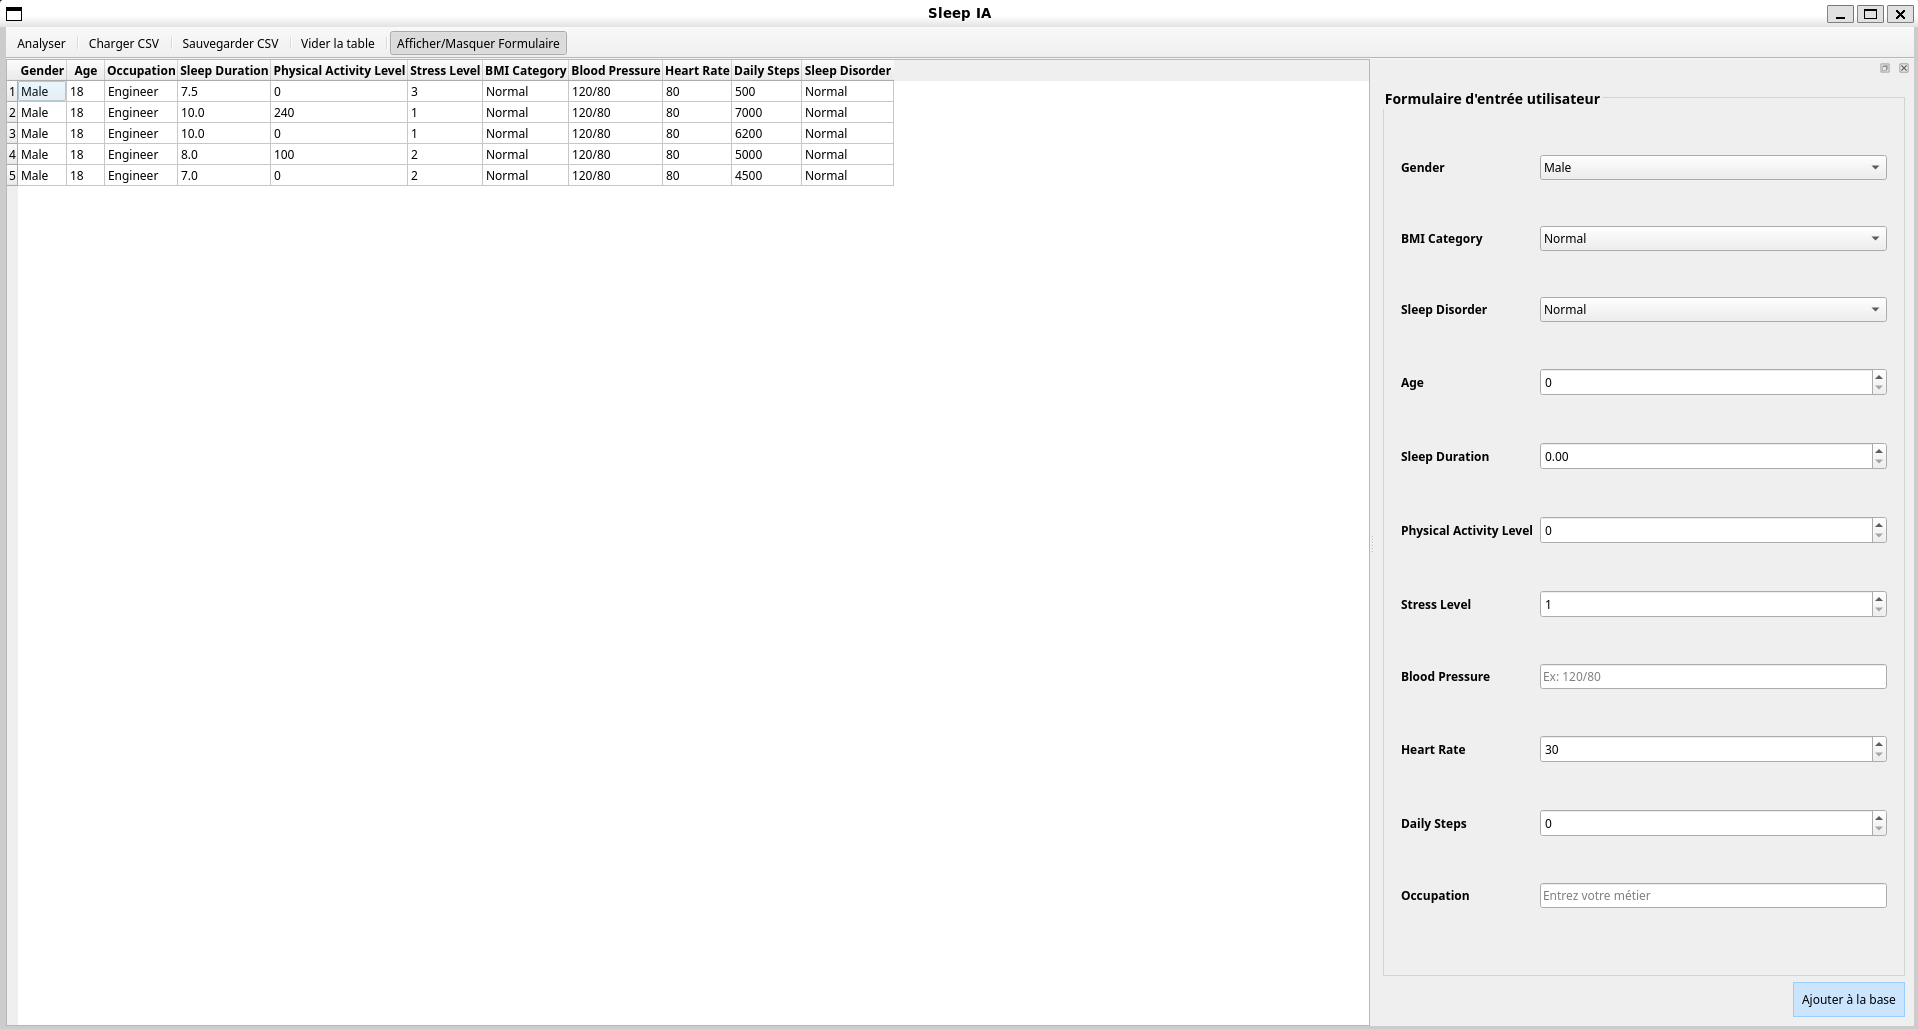
\includegraphics[width=0.7\textwidth]{screen_UI.png}
    % Capture d'écran de ton interface
  \end{center}
\end{frame}

\section{Discussion}

\begin{frame}{Limites et perspectives}
  \begin{itemize}
    \item Données : biais déclaratifs, petit volume
    \item Modèle : simple, améliorable (optimisation, régularisation)
    \item Pistes :
    \begin{itemize}
      \item Utilisation de séries temporelles
      \item Capteurs connectés (IoT santé)
    \end{itemize}
  \end{itemize}
\end{frame}

\begin{frame}{Conclusion}
  \begin{itemize}
    \item IA efficace pour prédire la qualité du sommeil
    \item Lien clair avec cycles biologiques et boucles d'IA
    \item Outil personnalisable avec application concrète
  \end{itemize}
  \vfill
  \centering{\textit{Merci pour votre attention !}}
\end{frame}

\end{document}
